% #####################################################################
% #####################################################################
% ##                                                                 ##
% ##                             Lizenz:                             ##
% ##                         CC BY-NC-SA 3.0                         ##
% ##      http://creativecommons.org/licenses/by-nc-sa/3.0/de/       ##
% ##                                                                 ##
% #####################################################################
% ##   Diese Datei kann beliebig verändert werden, solange darauf    ##
% ##     hingewiesen wird, dass dieses Dokument ursprünglich von     ##
% ##                                                                 ##
% ##                        www.ei-studium.de                        ##
% ##                                                                 ##
% ##                             stammt.                             ##
% ## Dies gilt insbesondere auch für alle daraus erstellten Dateien. ##
% ##    Des Weiteren muss die Weitergabe dieser Dateien unter der    ##
% ##                    gleichen Lizenz erfolgen.                    ##
% #####################################################################
% #####################################################################
\documentclass[a4paper,twocolumn,10pt]{article}
\usepackage[utf8]{inputenc}
\usepackage[ngerman]{babel}
\usepackage[top=2.0cm,bottom=1.5cm,left=1.0cm,right=1.0cm]{geometry}
\usepackage{enumitem}
\usepackage{graphicx}
\usepackage{amsfonts}
\usepackage{amsmath}
\usepackage{sectsty}
\usepackage{colortbl}
\usepackage{cancel}
\usepackage{listings}
\usepackage{color}
\usepackage{epstopdf}
\usepackage{fancyhdr}
\usepackage[pdfborder={0 0 0}]{hyperref}

\setlist{itemsep=.01mm}
\setenumerate{label=\emph{\arabic*})}
\setlength{\columnsep}{1cm}
\parindent 0mm

\partfont{\huge}
\sectionfont{\Large \sc\bf}
\subsectionfont{\normalsize}
\subsubsectionfont{\small\textit}

\pagestyle{fancy}
\lhead[\leftmark]{Digitaltechnik}
\chead[\leftmark]{\url{http://www.ei-studium.de}}
\rhead[\leftmark]{Erstelldatum: \today}
\lfoot[\leftmark]{Keine Garantie auf Vollständigkeit und Richtigkeit!}
\cfoot[\leftmark]{}
\rfoot[\leftmark]{\thepage}
\renewcommand{\headrulewidth}{0.5pt}
\renewcommand{\footrulewidth}{0.5pt}

\newcommand{\sollsein}{\stackrel{!}{=}}
\DeclareMathOperator{\val}{val}
\definecolor{tblgray}{gray}{.80}

\begin{document}

\part*{Digitale Schaltungen}

\section*{Zahlensysteme}

\subsection*{Größte darstellbare Zahl nach Anzahl der Ziffern}
b: Basis; p: Anz. Vorkommast.; n: Anz. Nachkommast.\\\\
$Z_{max}=b^p-b^{-n}$

\subsection*{Zahlenkonvertierung Dezimal nach Basis r}
Sei $z$ Zahl im Dezimalsystem.

\underline{Für $z \geq 1$}
\begin{enumerate}
	\item Teile $z$ durch $r$. Rest ist letzte Ziffer (LSB).
	\item Wiederhole mit Ergebnis von 1). Rest ist vorletzte Ziffer usw.
	\item letzter Rest ist erste Ziffer (MSB).
\end{enumerate}

\underline{Für $z<1$}
\begin{enumerate}
	\item Multipliziere $z$ mit $r$. Übertrag ist erste Ziffer (MSB).
	\item Wiederhole mit Ergebnis von 1). Übertrag ist zweite Ziffer usw.
	\item letzter Rest ist letzte Ziffer (LSB).
\end{enumerate}
Anzahl der benötigten Ziffern n bezüglich der Basis r, um $Z_{10}$ darstellen zu können:\\\\
$n=\lfloor log_r(Z)\rfloor +1$

\subsection*{Negative Zahl bilden (2er Komplement, Radix)}
$K(Z)=r^n-Z$
\begin{enumerate}
	\item Betrag der Dezimalzahl in Binärsystem umwandeln
	\item Binäre Zahl invertieren
	\item Anschließend 1 addieren
\end{enumerate}

\subsection*{Binäre Rechenoperationen}
$n_1$: Bit-Anzahl von Zahl 1; $n_2$: Bit-Anzahl von Zahl 2\\
Maximale Anzahl an Bit, um Ergebnis darzustellen:\\\\
Addition: $n_E=max(n_1,n_2)+1$\\
Multiplikation: $n_E=n_1+n_2$

\subsection*{Gleitkommazahlen (IEEE 754)}
1 bit Vorzeichen(v), 8 bit Exponent(e), 23 bit Mantisse(m)
\subsubsection*{Dezimalzahl $\rightarrow$ IEEE 754}
$Z$ positiv $\Rightarrow v=0;\;\;\;\;Z$ negativ $\Rightarrow v=1$\\\\
$e_{10}=\lfloor \log_2|Z_{10}| \rfloor+127\;\;\;\;\;\;\;\;\;m_{10}= \lfloor(\frac{|Z_{10}|}{2^{e_{10}-127}}-1)\cdot 2^{23}\rfloor$

\subsubsection*{IEEE 754 $\rightarrow$ Dezimalzahl}
$Z_{10}=(-1)^v\cdot (\frac{m_{10}}{2^{23}}+1)\cdot 2^{e_{10}-127}$\\\\
$Z_2=(-1)^v\cdot(1,m_2)\cdot 2^{e_{10}-127}$\\\\
\begin{tabular}{@{}l@{}l}
$e=0$ & $\;\;\Rightarrow$Darstellung von ,,0''\\
$e=255$ & $\;\;\Rightarrow$Darstellung von ,,$\infty$''
\end{tabular}

\section*{MOSFET-Transistor}
\subsection*{nMOS}
\begin{minipage}[b]{0.35\textwidth}
Guter Pull-Down\\
Source am niedrigeren Potential ($U_{DS} > 0$)
\end{minipage}
\hfill
\begin{minipage}[b]{0.1\textwidth}
\centering
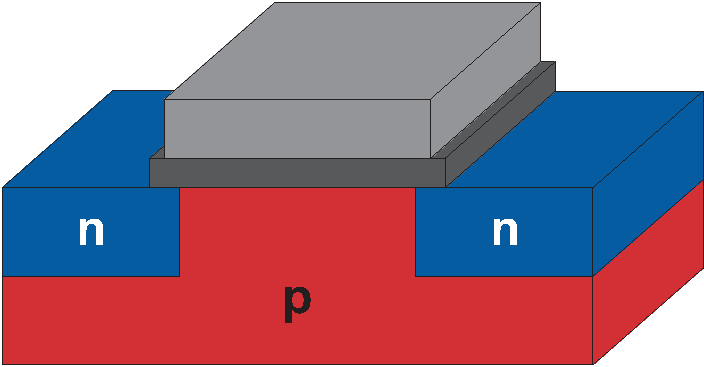
\includegraphics[width=\textwidth]{Grafiken/nMOS}
\end{minipage}
\begin{itemize}[label=,leftmargin=0mm]
	\item $I_D=\begin{cases}
				0 & U_{GS} < U_t (aus) \\
				& \wedge \; U_{DS} \geq 0 \\
				\beta\left(U_{GS}-U_t-\frac{U_{DS}}{2}\right)U_{DS} & U_{GS} > U_t $ (linear)$ \\
				& \wedge \;0 < U_{DS} < U_{GS}-U_t \\
				\frac{\beta}{2}\left(U_{GS}-U_t\right)^2 & U_{GS} > U_t $ (Sättigung)$\\
				& \wedge \;0 < U_{GS}-U_t < U_{DS} \\
			\end{cases}$
\end{itemize}

\subsection*{pMOS}
\begin{minipage}[b]{0.35\textwidth}
Guter Pull-Up\\
Source am höheren Potential ($U_{DS} < 0$)
\end{minipage}
\hfill
\begin{minipage}[b]{0.1\textwidth}
\centering
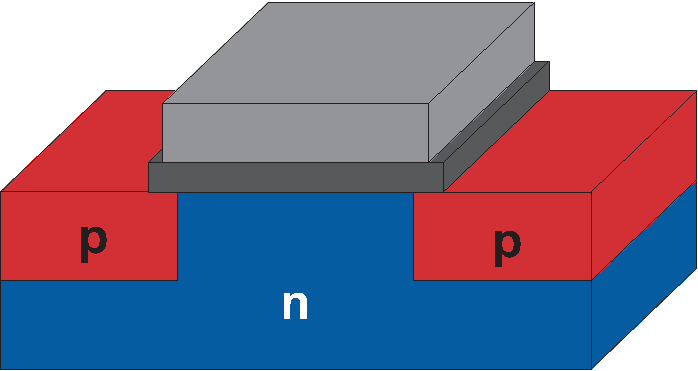
\includegraphics[width=\textwidth]{Grafiken/pMOS}
\end{minipage}
\begin{itemize}[label=,leftmargin=0mm]
	\item $I_D=\begin{cases}
				0 & U_{GS} > U_t (aus) \\
				& \wedge \; U_{DS} \leq 0 \\
				-\beta\left(U_{GS}-U_t-\frac{U_{DS}}{2}\right)U_{DS} & U_{GS} < U_t $ (linear)$ \\
				& \wedge \;0 > U_{DS} > U_{GS}-U_t \\
				\frac{-\beta}{2}\left(U_{GS}-U_t\right)^2 & U_{GS} < U_t $ (Sättigung)$\\
				& \wedge \;0 > U_{GS}-U_t > U_{DS} \\
			\end{cases}$
\end{itemize}

\subsection*{Dimensionierung}
\begin{minipage}[b]{0.2\textwidth}
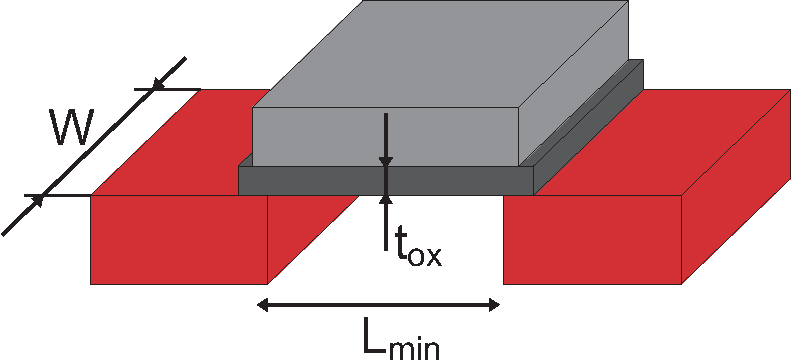
\includegraphics[width=\columnwidth]{Grafiken/Dimensionierung}
\end{minipage}
\hfill
\begin{minipage}[b]{0.3\textwidth}
$\;\;\beta=K'\frac{W}{L}$ mit $K'=\frac{\mu\varepsilon_{Ox}\varepsilon_0}{t_{Ox}}$
\end{minipage}
\begin{tabbing}
$\varepsilon_{Ox}$: \= rel. Dielektrizitätskonstante des Gate Oxyds \\
$\varepsilon_0$: \> Dielektrizitätskonstante \\
$W$: \> Kanalweite    $L$: Kanallänge \\
$\mu$: \> Beweglichkeit der Elektronen/Löcher \\
$t_{Ox}$: \> Gate Oxyd-Dicke
\end{tabbing}
\begin{enumerate}[label=,leftmargin=0mm]
	\item $L$ immer $L_{min}$
	\item $W \sim $ Drain Strom $\sim$ Schaltgeschwindkeit
	\item $\mu_n=(1.5\ldots 3.5)\cdot \mu_p \Rightarrow$ Kanalweite bei pMOS größer
	\item $\Rightarrow$ nMOS schaltet prinzipiell schneller als pMOS
\end{enumerate}

\subsection*{Verzögerungszeit (Propagation delay)}
Zeit zwischen 50\%-Pegeln von Eingang und Ausgang.\\\\
$t_p=R_{on,p}\cdot C\cdot \ln(2)$ , $R_{on,p}\approx\frac{1}{\beta(|U_{GSp}|-|U_{tp}|)}$
$t_{pLH} \sim \frac{C_{load}t_{Ox}L_p}{W_p\mu_p\varepsilon_{Ox}(U_{DD}-|U_{tp}|)}$
\newline\newline\newline
\begin{tabular}{p{0.48\columnwidth}|p{0.48\columnwidth}}
\multicolumn{1}{l}{\textbf{Zunahme von:}} \\
\hline
{
\setlength{\topsep}{0pt}
\begin{tabbing}
$C_{load}:$ \= Kapazitive Last\\
$t_{ox}:$ \> Oxiddicke\\
$L_p:$ \> Kanallänge\\
$U_{tp}:$ \> Schwellspannung \\
\> (Betrag)
\end{tabbing}
$\Rightarrow$ Verzögerungszeit steigt
}
 & 
{
\setlength{\topsep}{0pt}
\begin{tabbing}
$W_p:$ \= Kanalweite\\
$\mu_p:$ \> Beweglichkeit der \\
\> Ladungsträger\\
$\varepsilon_{ox}:$ \> Oxyd-Dielektrizität\\
$U_{DD}:$ Versorungsspannung
\end{tabbing}
$\Rightarrow$ Verzögerungszeit sinkt
}
\end{tabular}
\\\\
Beeinflussbare Parameter: $C_{load}, W_p, U_{DD}, U_{tp}$

\section*{CMOS-Inverter und Logik}
\subsection*{Verlustleistung}
\subsubsection*{Dynamisch}
Abhängig von den Signalflanken und der Schaltfunktion\\\\
\underline{Kapazitiver Anteil:}\\
Eingangskapazitäten nachfolgender Gatter, Leitungskapazitäten, parasitäre Kapazitäten\\\\
\underline{Kurzschlussanteil:}\\
Querstrom (aufgrund endlicher Flankensteilheit)

\subsubsection*{Statisch}
Sub-Schwellstrom, Leckstrom (Diodensperrstrom), Gate-Strom \\
 $\Rightarrow$ abhängig von Versorgungs- und Schwellspannung\\\\
 $P_{dyn} \approx P_{stat}$\\
$P_{Cap}=\alpha_{01}fCU_{dd}^2$\\
$P_{Short}=\alpha_{01}f\beta_n\tau(U_{dd}-2U_{tn})^2$\\\\
$\alpha = \frac{Anzahl\; der\; steigenden\; Flanken\; des\; Signals\ Z}{Anzahl\; der\; steigenden\; Flanken\; des\; Taktsignals}$\\\\
Falls Schaltwahrscheinlichkeit gegeben ist:\\\\
$\alpha = P(Z=0)\cdot P(Z=1)$

\subsection*{Singlecore vs. Multicore: dyn. Verlustleistung}
n: Anzahl der Kerne\\
k: um diesen Faktor verkürzte Laufzeit\\\\
Singlecore: $P_{dyn} \sim f\cdot U_{dd}^2$\\\\
Annahme: Programm kann perfekt parallelisiert werden.\\\\
Multicore: $P_{dyn} \sim \frac{k^3\cdot f \cdot U_{dd}^2}{n^2}$

\subsection*{Kennlinie von CMOS-Inverter}
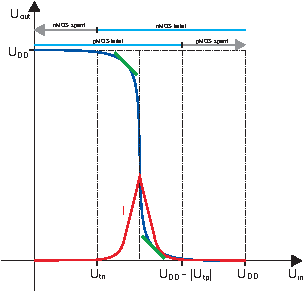
\includegraphics[width=0.36\textwidth]{Grafiken/Inverter_Kennlinie}\\\\
$v_{out}$ hat definierten Logikpegel, wenn gilt: $|\frac{\partial v_{out}}{\partial v_{in}}|<1$

\section*{Kombinatorische Logik}
\subsection*{Realisierung von CMOS-Schaltungen}
\begin{minipage}[b]{0.23\textwidth}
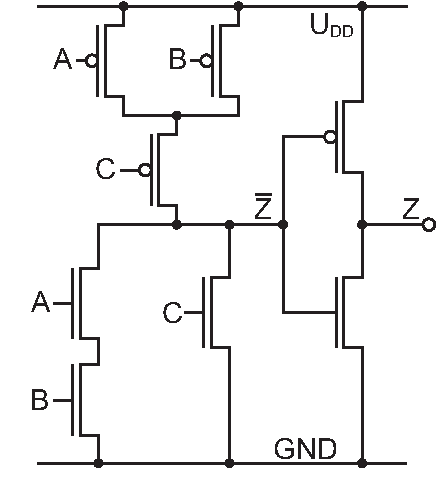
\includegraphics[width=0.95\textwidth]{Grafiken/CMOS-Schaltung}
\end{minipage}
\hfill
\begin{minipage}[b]{0.23\textwidth}
Beispiel: $Z=AB+C$\\\\\\
CMOS ist grundsätzlich invertierend!\\\\\\
\end{minipage}

\subsection*{DNF und KNF}
\begin{minipage}[b]{0.3\textwidth}
\begin{tabular}{@{}p{\textwidth}}
	\underline{DNF (= CSOP):}\\
	1-Zeilen mit ODER verknüpfen\\\\
	$Z=\overline{A}\cdot\overline{B}\cdot C+\overline{A}\cdot B\cdot\overline{C}+A\cdot\overline{B}\cdot\overline{C}+A\cdot B\cdot C$ \\\\
	\underline{KNF (= POS):}\\
	Werte der 0-Zeilen invertieren und mit UND verknüpfen
	\begin{tabbing}
	$Z=$ \= $(A+B+C)\cdot(A+\overline{B}+\overline{C})\cdot$ \\
	\> $\cdot(\overline{A}+B+\overline{C})\cdot(\overline{A}+\overline{B}+C)$
	\end{tabbing}
\end{tabular}
\end{minipage}
\hfill
\begin{minipage}[b]{0.16\textwidth}
\definecolor{Gray}{gray}{0.8}
\begin{tabular}{@{}|c|c|c|c|}
\hline \rowcolor{white} \textbf{A} & \textbf{B} & \textbf{C} & \textbf{Z} \\ 
\hline 0 & 0 & 0 & 0 \\ 
\hline \rowcolor{Gray} 0 & 0 & 1 & 1 \\
\hline \rowcolor{Gray} 0 & 1 & 0 & 1 \\
\hline \rowcolor{white}0 & 1 & 1 & 0 \\
\hline \rowcolor{Gray} 1 & 0 & 0 & 1 \\
\hline \rowcolor{white}1 & 0 & 1 & 0 \\
\hline 1 & 1 & 0 & 0 \\
\hline \rowcolor{Gray} 1 & 1 & 1 & 1 \\
\hline 
\end{tabular}
\end{minipage}

\subsubsection*{Umwandlung von SOP nach POS}
\begin{enumerate}
	\item Doppeltes Negieren der Funktion
	\item Umformung der unteren Negation (2x DeMorgan)
	\item Ausmultiplizieren
	\item Umformung der oberen Negation (2x DeMorgan)
\end{enumerate}

\subsection*{Volladdierer}
\begin{minipage}[b]{0.23\textwidth}
\centering
\begin{tabular}[b]{@{}|c|c|c|c|c|}
\hline \textbf{A} & \textbf{B} & \textbf{C$_{in}$} & \textbf{C$_{out}$} & \textbf{S} \\ 
\hline 0 & 0 & 0 & 0 & 0 \\ 
\hline 0 & 0 & 1 & 0 & 1 \\
\hline 0 & 1 & 0 & 0 & 1 \\
\hline 0 & 1 & 1 & 1 & 0 \\
\hline 1 & 0 & 0 & 0 & 1 \\
\hline 1 & 0 & 1 & 1 & 0 \\
\hline 1 & 1 & 0 & 1 & 0 \\
\hline 1 & 1 & 1 & 1 & 1 \\
\hline 
\end{tabular}
\end{minipage}
\hfill
\begin{minipage}[b]{0.27\textwidth}
\centering
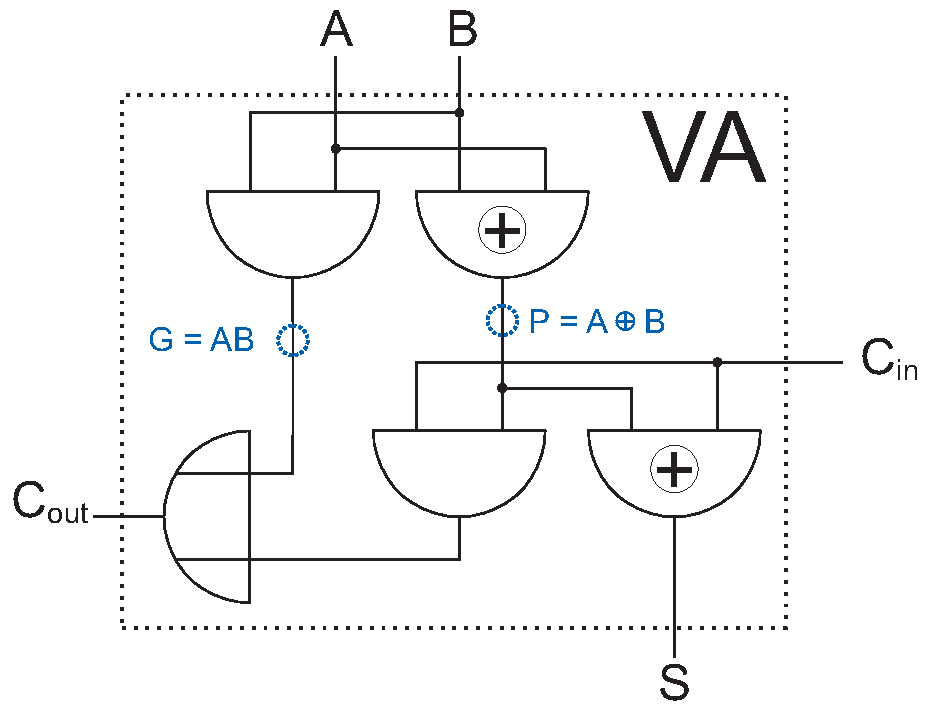
\includegraphics[width=\textwidth]{Grafiken/Volladdierer}
\end{minipage}
$S=P\oplus C_{in}\;,\;\; C_{out}=G+P\cdot C_{in}$ 

\subsection*{Ripple-Carry-Adder}
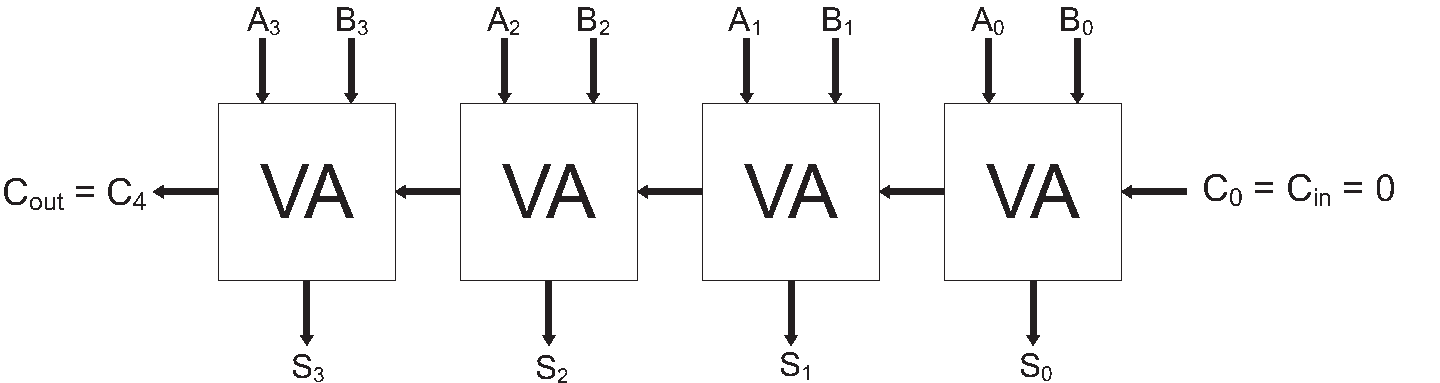
\includegraphics[width=0.5\textwidth]{Grafiken/Ripple-Carry}
Verzögerungszeit wird vom Carry-Übertrag dominiert!\\
Maximale Verzögerungszeit, wenn beim LSB das Signal von G wechselt und bei allen anderen Gattern gilt: $P=1$.

\section*{Sequentielle Logik}
\subsection*{Set-Reset Latch / Enable Latch}
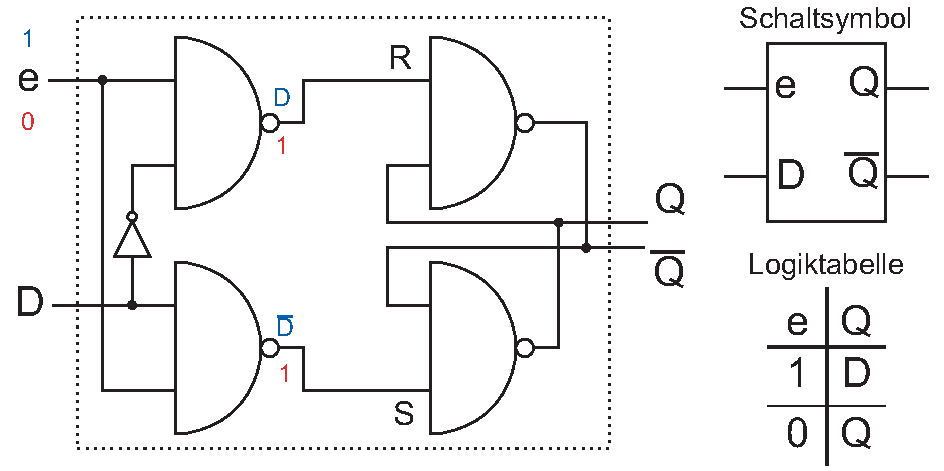
\includegraphics[width=0.4\textwidth]{Grafiken/SRLatch}
Übernimmt Eingangswert, solange e = 1 (Level-controlled)

\subsection*{Flip-Flop}
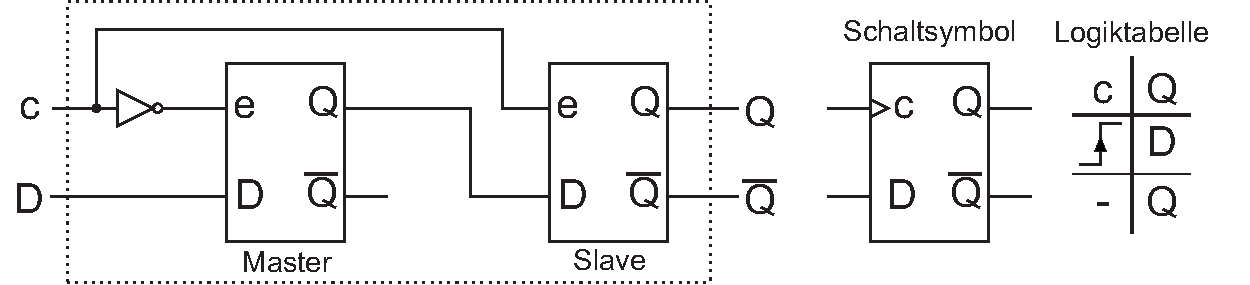
\includegraphics[width=0.5\textwidth]{Grafiken/FlipFlop}

\subsection*{Timing}
\begin{enumerate}[label=,leftmargin=0mm]
	\item \textbf{$t_{setup}$}: Zeit, in der der Eingangswert vor aktiver Taktflanke stabil sein muss
	\item \textbf{$t_{hold}$}: Zeit, in der der Eingangswert nach aktiver Taktflanke stabil bleiben muss
	\item \textbf{$t_{c2q}$}: Zeit, nach der der Eingangswert nach der Taktflanke stabil an Q anliegt (=Ausgangslatenz des Registers)
	\item \textbf{$t_{clk}$}: Clock
	\item \textbf{$t_{l"angsterPfad}$}: (=kritischer Pfad) Längste Verzögerungszeit zwischen zwei Registerstufen
\end{enumerate}

\fbox{$t_{clk} \geq t_{c2q} + t_{l"angster Pfad} + t_{setup}$}
\fbox{$t_{hold} \leq t_{c2q}+t_{k"urzester Pfad}$}\\\\
$f_{max}=\frac{1}{t_{setup}+t_{c2q}+t_{l"angsterPfad}}$\\\\
(Für maximalen Durchsatz die Einheit \glqq op/s\grqq\;verwenden!)\\\\
$Gesamtlatenz=($Maximale Anzahl hintereinander geschalteter Register $-1)\cdot t_{clk}$\\\\
Für eine dauerhaft korrekte Datenübergabe müssen alle Register mit der selben Frequenz arbeiten (ansonsten: Verletzung der Hold-/Setup-Zeit usw.).

\subsection*{Pipelining}
Aufteilen langer kombinatorischer Pfade durch Einfügen zusätzlicher Registerstufen, um die Taktfrequenz erhöhen zu können (Gesamtlatenz wird allerdings nicht kleiner).\\
$\Rightarrow$ Möglichst Halbierung des längsten Pfades!\\
$\Rightarrow$ Evtl. müssen sog. \glqq Dummy-Gatter\grqq\; eingefügt werden!

\subsection*{Parallele Verarbeitungseinheiten}
\begin{enumerate}[label=-,leftmargin=5mm]
	\item Paralleles, gleichzeitiges Verwenden mehrere identischer Schaltnetze
	\item Zusätzliche Kontrolllogik nötig (Multiplexer)
	\item Taktfrequenz und Latenz bleiben konstant
	\item Durchsatz steigt mit der Zahl der Verarbeitungseinheiten
	\item ABER: deutlich höherer Ressourcenverbrauch
\end{enumerate}

\subsection*{Finite state machine}
\begin{tabular}{p{0.45\columnwidth} p{0.50\columnwidth}}
\textbf{Moore} & \textbf{Mealy}\\ \\
\end{tabular}
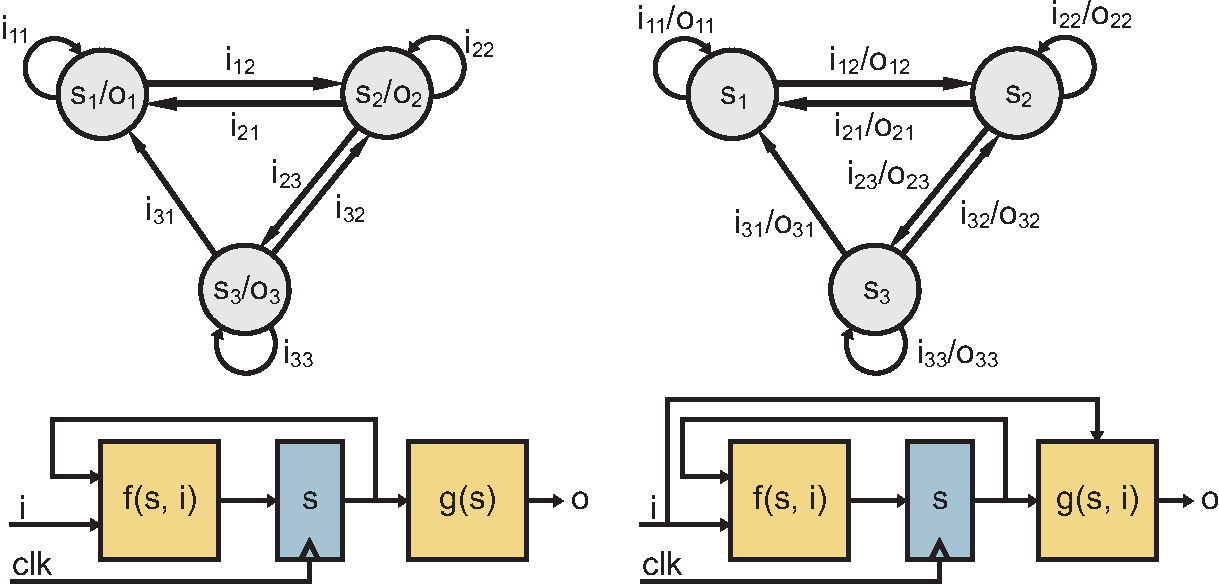
\includegraphics[width=0.5\textwidth]{Grafiken/MooreMealy}
\newline\newline
\begin{tabular}{p{0.50\columnwidth} p{0.50\columnwidth}}
Ausgang nur vom Zustand abhängig. & Ausgang vom Zustand und von Eingabe abhängig.\\ \\
\end{tabular}
\begin{tabular}{p{0.50\columnwidth}|p{0.50\columnwidth}}
\multicolumn{1}{l}{\textbf{Vorteile:}} \\
\hline
Kein Kombinatorischer Pfad von Eingängen zu Ausgängen 
\begin{tabbing}
$\Rightarrow$ \= Begrenzung der Logik-\\
\> Tiefe
\end{tabbing} & Weniger Zustände, Übersichtlicher, Allgemeiner \\
\multicolumn{1}{l}{\textbf{Nachteile:}} \\
\hline
Hohe Anzahl von Zuständen & 
Lange kombinatorische Pfade bei Vekettung mehrerer FSMs
\end{tabular}

\section*{Speicher}
\subsection*{Definitionen}
\begin{tabbing}
\textit{Bandbreite:} \= Datenmenge pro Zeiteinheit zum Schreiben \\
\> oder Lesen [bit/sec]\\
\textit{Latenz:} \> Zeitdifferenz zwischen Anforderung und \\
\> Ausgabe von Daten [sec]\\
\textit{Zykluszeit:} \> Zeitdifferenz zwischen auffeinander folgenden \\
\> Schreib/Lese Zyklen [sec]\\
\textit{Asynchron:} \> Lese-/Schreibvorgang beginnt direkt \\
\> $\Rightarrow$ \= neues Datenwort kann unmittelbar am \\
\> \> Ausgang anliegen\\
\textit{Synchron:} \> Fester Systemtakt ($\rightarrow$ Fließbandverarbeitung)\\
\> $\Rightarrow$ Datenwort ist frühestens mit nächstem Takt \\
\> \> nach Anlegen einer neuen Adresse zu erwarten \\
\end{tabbing}
Bei der Anordnung von Speicherzellen in Reihen und Spalten wird darauf geachtet, dass es möglichst quadratisch ist.\\\\
Leseverstärker zwischen Speicherzelle und Decoder beschleunigen den Speicherzugriff.

\subsection*{1-Transistor DRAM-Zelle}
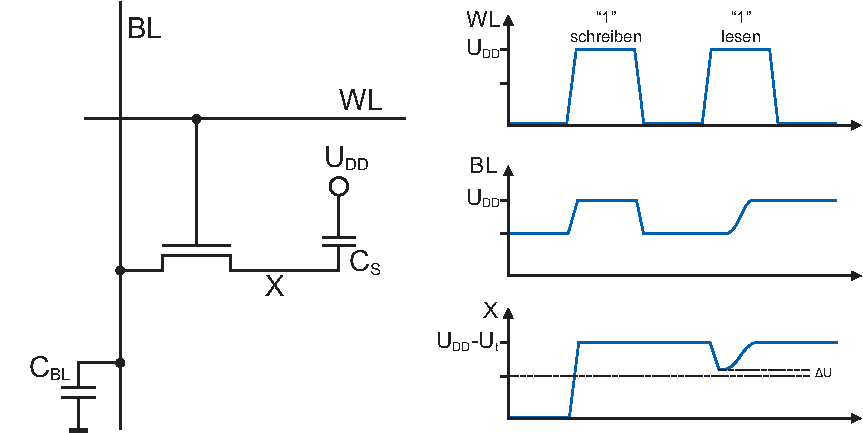
\includegraphics[width=0.4\textwidth]{Grafiken/1-Transistor-DRAM}
\begin{flushright}
$\Delta U=(U_X-\frac{U_{DD}}{2})\cdot \frac{C_S}{C_S+C_{BL}}$
\end{flushright}
Signalverstärkung und Refresh-Zyklen notwendig.

\subsection*{6-Transistor SRAM-Zelle}
\begin{center}
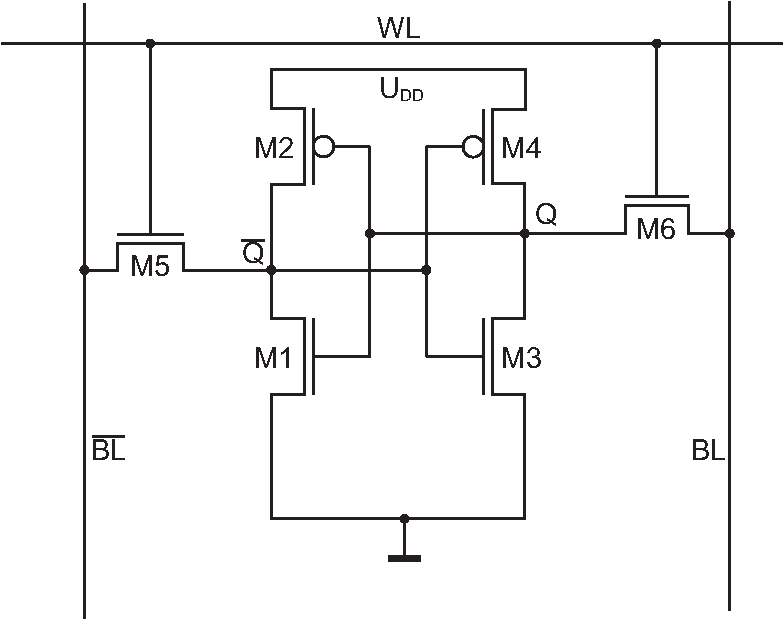
\includegraphics[width=0.35\textwidth]{Grafiken/6-Transistor-SRAM}
\end{center}
Die Transitoren M1 - M4 realisieren ein CMOS-Latch zur Speicherung einer "0" bzw. "1".
Über die Transistoren M5 und M6 wird die Speicherzelle zum Lesen oder Schreiben ausgewählt.

\subsection*{Flash}
\begin{center}
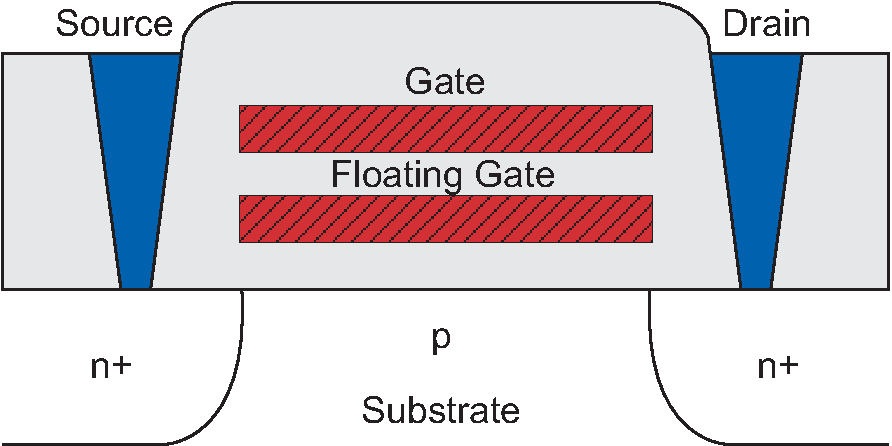
\includegraphics[width=0.25\textwidth]{Grafiken/Flash}
\end{center}
\subsubsection*{Lesen}
Information sitzt auf dem Floating Gate. Je nach Zustand (1/0) sitzen dort Ladungsträger oder nicht.
Evtl. vorhandene Ladungsträger bewirken eine Änderung der Schwellspannung des Transistors, der bei Anlegen einer Gatespannung je nach Speicherzustand durchschaltet oder nicht.

\subsubsection*{Schreiben}
An Gate und Drain wird eine hohe Programmierspannung angelegt (Source auf GND).
Dadurch werden die Elektronen stärker beschleunigt als normal und tunneln zum Floating Gate.

\subsubsection*{Löschen}
An Drain wird eine hohe Spannung und an Gate GND angelegt (Source von GND abgetrennt).
Die Elektronen werden dadurch von Drain abgezogen (tunneln durch das Oxyd).

\part*{EDS}

\section*{Algebra}
\subsection*{Boolesche Algebra}
\begin{enumerate}
	\item $x\cdot y=y\cdot x, x+y=y+x$
	\item $(x\cdot y)\cdot z=x\cdot (y\cdot z)\;,\;\;(x+y)+z=x+(y+z)$
	\item $x\cdot (y+z)=x\cdot y+x\cdot z$
	\item $x\cdot x=x\;,\;\; x+x=x$
	\item $x\cdot (x+y)=x\;,\;\; x+x\cdot y=x$
	\item $1\cdot x=x\;,\;\; 0+x=x$
	\item $0\cdot x=0\;,\;\; 1+x=1$
	\item $x\cdot \overline{x}=0\;,\;\; x+\overline{x}=1$
	\item $\overline{\overline{x}}=x$
	\item $\overline{x\cdot y}=\overline{x}+\overline{y}\;,\;\; \overline{x+y}=\overline{x}\cdot \overline{y}$
\end{enumerate}

\subsection*{XOR Algebra}
\begin{enumerate}
	\item $x\oplus y=y\oplus x$
	\item $(x\oplus y)\oplus z=x\oplus (y\oplus z)$
	\item $x\cdot (y\oplus z)=x\cdot y\oplus x\cdot z$
	\item $x\oplus 0=x$
	\item $\overline{x}=x\oplus 1\;,\;\; \overline{x\oplus y}=x\oplus y\oplus 1$
	\item $x\oplus\overline{x}=1\;,\;\; x\oplus x=0$
	\item $x\oplus x\oplus x=x$
	\item $x\oplus y=\overline{x}\oplus\overline{y}$
	\item $x\oplus y=x\cdot\overline{y}+\overline{x}\cdot y$
	\item $x\oplus y=(x+y)\cdot(\overline{x}+\overline{y})$
	\item $x+y=x\oplus y\oplus x\cdot y$
	\item $x\cdot y=x\oplus y\oplus (x+y)$
\end{enumerate}

\section*{Schaltsymbole}
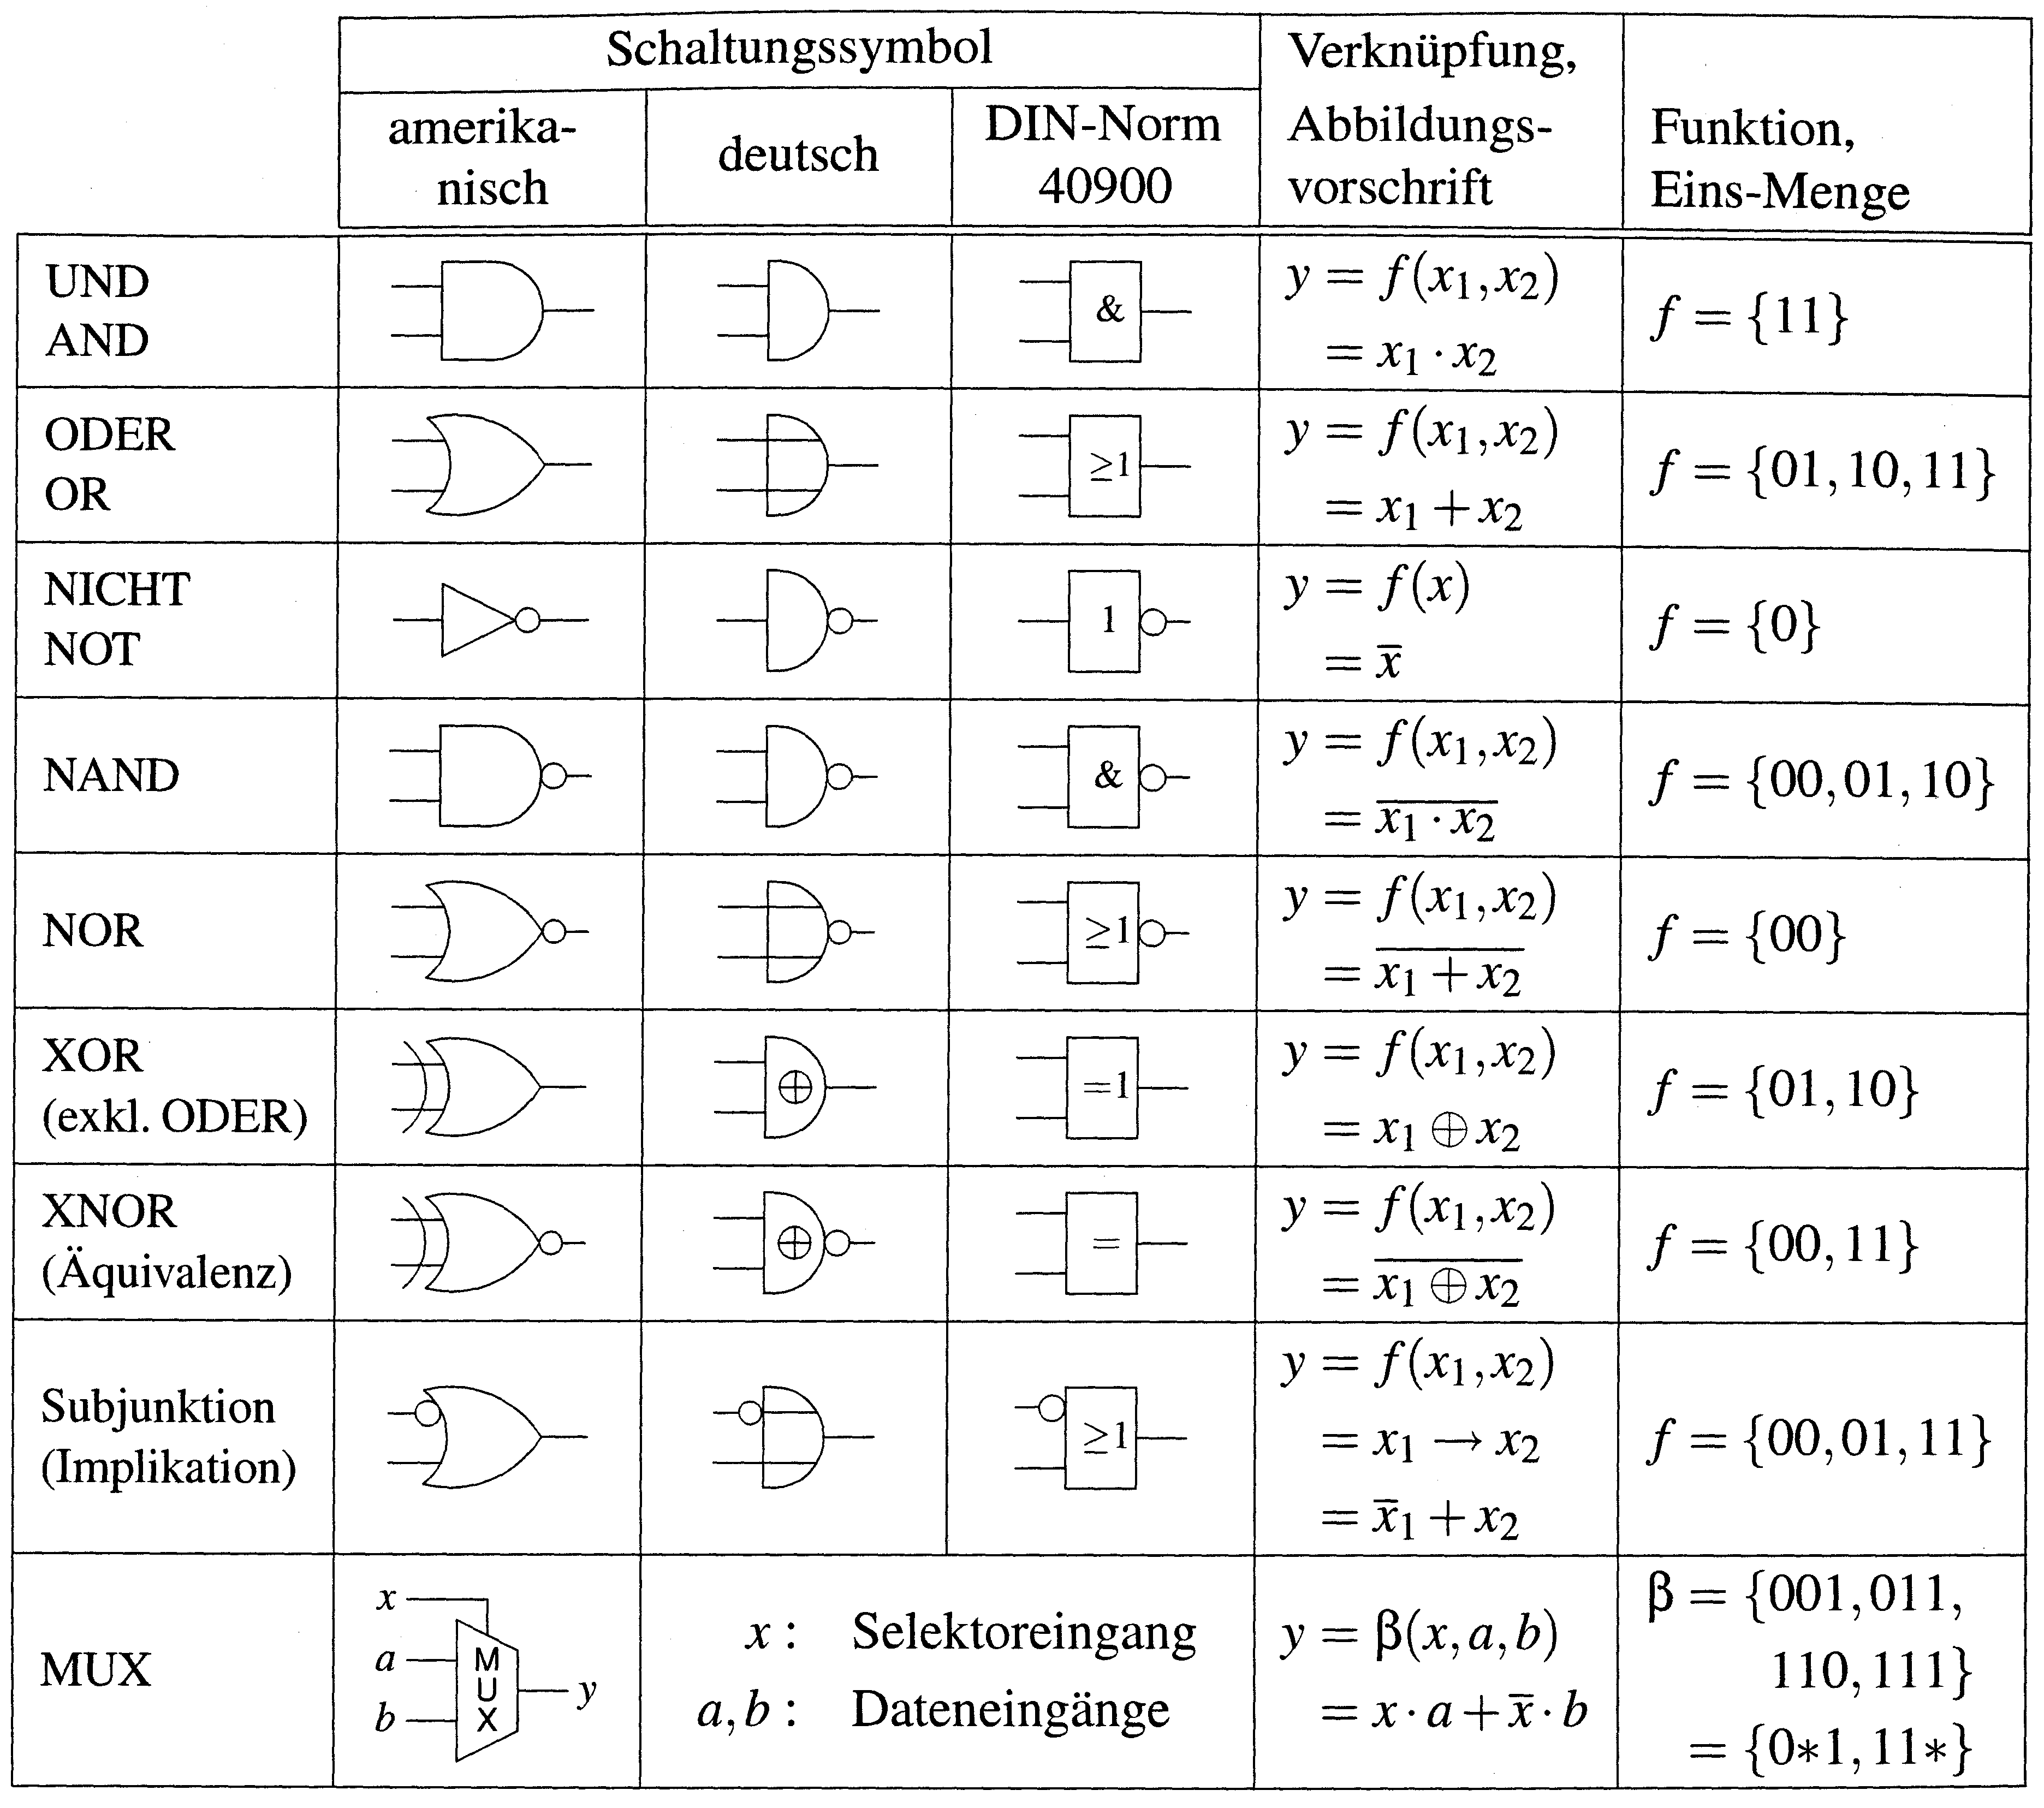
\includegraphics[width=0.5\textwidth]{Grafiken/Schaltsymbole}

\section*{Binäre Boolsche Funktionen}
\subsection*{Kofaktor}
	\begin{itemize}[label=-]
	\item $f|_{x_i=1}=f_{x_i}\;,\;\; f|_{x_i=0}=f_{\overline{x}_i}$
	\item $(f_{x_i})_{x_j}=(f_{x_j})_{x_i}=f_{x_ix_j}$
	\item $x_i\cdot f=x_i\cdot f_{x_j}\;,\;\; \overline{x}_i\cdot f=\overline{x}_i\cdot f_{\overline{x}_j}$
	\item $x_i + f=x_i + f_{\overline{x}_j}\;,\;\; \overline{x}_i+f=\overline{x}_i+f_{x_j}$
\end{itemize}

\subsection*{Entwicklungssätze}
\begin{enumerate}[label=-]
	\item $f=x_i\cdot f_{x_i}+\overline{x}_i\cdot f_{\overline{x}_i}=\beta(x_i, f_{x_i}, f_{\overline{x}_i})$
	\item $\overline{f}=x_i\cdot \overline{f_{x_i}}+\overline{x}_i\cdot \overline{f_{\overline{x}_i}}$
\end{enumerate}
\subsection*{Sonstiges}
\begin{enumerate}[label=-]
	\item $f$ unabhängig von $x_i \Leftrightarrow f_{x_i}=f_{\overline{x}_i}\Leftrightarrow f_{x_i}\oplus f_{\overline{x}_i}=0$
	\item $f$ abhängig von $x_i \Leftrightarrow f_{x_i}\neq f_{\overline{x}_i}\Leftrightarrow f_{x_i}\oplus f_{\overline{x}_i}=1$
	\item $f$ positiv symmetrisch in $x_i$ und $x_j \Leftrightarrow f_{x_i\overline{x}_j}=f_{\overline{x}_ix_j}$
	\item $f$ negativ symmetrisch in $x_i$ und $x_j \Leftrightarrow f_{x_ix_j}=f_{\overline{x}_i\overline{x}_j}$
\end{enumerate}

\section*{Kubengraphen}
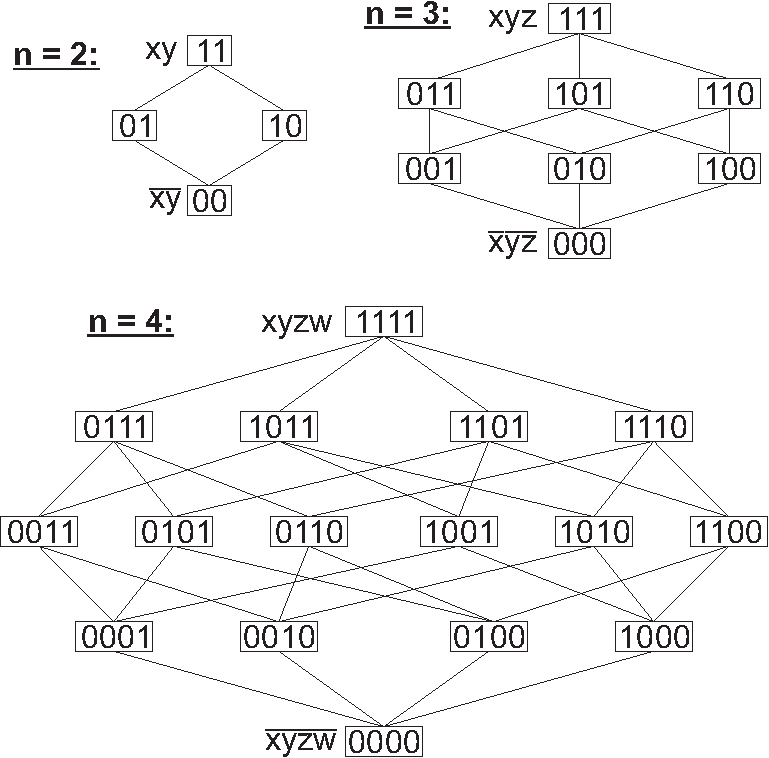
\includegraphics[width=0.42\textwidth]{Grafiken/Kubengraphen}\\\\\\
Menge aller Knoten (0-Kuben) $=2^n$\\
Menge aller Kuben $=3^n$\\
Menge aller Kanten $=\frac{n}{2}\cdot 2^n$\\\\
Kubenabstand $\delta(c_1,c_2)$:\\
Anzahl($\#$) an Literalen, die in $c_1$ negiert und in $c_2$ nicht negiert vorkommen und umgekehrt.\\
$\#$Kubusliterale = $\#$Raumdimensionen - $\#$Kubusdimension\\
$\#$Überdeckte Minterme = $2^{Kubusdimension}$

\section*{Begriffe}
\subsection*{Cover}
z.B.: $f=y\cdot z+\overline{x}\cdot y+\overline{x}\cdot\overline{y}$\\\\
$\Rightarrow cov(f)=\{y\cdot z, \overline{x}\cdot y, \overline{x}\cdot\overline{y}\}$


\section*{MinSOP nach Quine/McCluskey}
\subsection*{Nachteile}
\begin{enumerate}[leftmargin=6mm]
\item Benötigt CSOP als Eingangsform
\item Länge wächst exponentiell mit Dimension
\end{enumerate}

\subsection*{Gesetze}
\subsubsection*{Spezielles Resolutionsgesetz}
$x\cdot a + \overline{x}\cdot a=a$

\subsubsection*{Absorptionsgesetz} $a+a\cdot b=a\\$

\subsection*{Minimierungstabelle}
\begin{tabular}{|c|c|c|c|c|c|}
\hline $m_i$ & 0-Kubus & A & 1-Kubus & A & \ldots \\ 
\hline $m_0$ & $\overline{x}\cdot\overline{y}\cdot\overline{z}$ & \checkmark  & $\overline{x}\cdot\overline{z}$ & &  \\ 
\hline $m_2$ & $\overline{x}\cdot y\cdot\overline{z}$ & \checkmark  & $\overline{x}\cdot y$ & &  \\ 
\hline $m_3$ & $\overline{x}\cdot y\cdot z$ & \checkmark  & $y\cdot z$ & &  \\ 
\hline $m_7$ & $x\cdot y\cdot z$ & \checkmark  &  &  &  \\ 
\hline 
\end{tabular}
$\\ \Rightarrow$ VollSOP : $f=\overline{x}\cdot\overline{z}+\overline{x}\cdot y+y\cdot z=p_1+p_2+p_3 \\$

\subsection*{Minimierung der Primimplikanten}
\subsubsection*{Algebraisch}
$C=(m_0\subset p_1)\cdot(m_2\subset p_1+m_2\subset p_2)\cdot(m_3\subset p_2+m_3\subset p_3)\cdot(m_7\subset p_3)
\\C=\tau_1\cdot(\tau_1+\tau_2)\cdot(\tau_2+\tau_3)\cdot\tau_3\sollsein 1
\\C=\tau_1\cdot\tau_3+\tau_1\cdot\tau_2\cdot\tau_3
\\C=\tau_1\cdot\tau_3\\$

\subsubsection*{Überdeckungstabelle}
\begin{tabular}{|c|c|c|c|c|}
\hline $p \backslash m$ & $m_0$ & $m_2$ & $m_3$ & $m_7$ \\ 
\hline $p_1$ & \cellcolor{tblgray}1 & \cellcolor{tblgray}1 & 0 & 0 \\ 
$p_2$ & 0 & 1 & 1 & 0 \\ 
$p_3$ & 0 & 0 & \cellcolor{tblgray}1 & \cellcolor{tblgray}1 \\ 
\hline 
\end{tabular}\\\\
$\Rightarrow$ MinSOP : $f=p_1+p_3=\overline{x}\cdot\overline{z}+y\cdot z$

\section*{Resolventenmethode}
\subsection*{Gesetze}
\subsubsection*{Allgemeines Resolutionsgesetz}
$x\cdot a + \overline{x}\cdot b=x\cdot a + \overline{x}\cdot b + a\cdot b$

\subsubsection*{Absorptionsgesetz}
$a+a\cdot b=a$\\

\begin{tabular}{|l|c|}
\hline $f$ & Schicht \\ 
\hline $\overline{x}\cdot y+\cancel{x\cdot y\cdot z} + \cancel{\overline{x}\cdot\overline{y}\cdot\overline{z}}$ & 0 \\ 
\hline $+ y\cdot z+\overline{x}\cdot\overline{z}$ & 1 \\ 
\hline 
\end{tabular}

\section*{Mehrfachimplikanten}
Implikanten, die in mehreren Funktionen vorhanden sind, können gemeinsam genutzt werden.\\
$\Rightarrow$ Nur sinnvoll, wenn dadurch die Gesamtliteralzahl sinkt.
\begin{enumerate}
	\item Zur Vereinfachung MinSOP von $f_1, f_2,...$ bestimmen
	\item Mehrfachimplikant $=f_1\cdot f_2\cdot ...$
\end{enumerate}

\section*{Karnaugh-Diagramm}
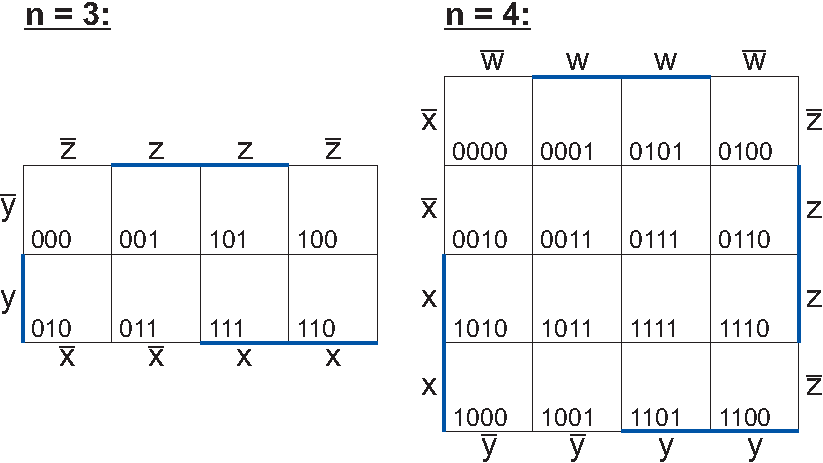
\includegraphics[width=0.45\textwidth]{Grafiken/Karnaugh}

\section*{Heuristische Minimierung}
\subsection*{Literalentfernung (expand)}
z.B.: Dürfen $\overline{y}$ und $\overline{z}$ aus $\overline{y} \cdot\overline{z} \cdot\overline{w}$ einzeln bzw. gemeinsam entfernt werden?
\begin{enumerate}[label=-]
	\item $\overline{y}$ darf entfernt werden, falls $f_{y \cdot\overline{z} \cdot\overline{w}}=1$
	\item $\overline{z}$ darf entfernt werden, falls $f_{\overline{y} \cdot z \cdot\overline{w}}=1$
	\item $\overline{y}$ und $\overline{z}$ dürfen entfernt werden, falls $f_{y \cdot z \cdot\overline{w}}=1$
\end{enumerate}

\subsection*{Kubenentfernung (remove)}
z.B.: Darf der Kubus $\overline{x}w$ von $f$ entfernt werden?
\begin{enumerate}
	\item $\Rightarrow \overline{x}w$ von $f$ entfernen $\rightarrow h$
	\item $\overline{x}w$ darf entfernt werden, falls $h_{\overline{x}w}=1$
\end{enumerate}

\subsection*{Literalzahlerhöhung (reduce)}
$\rightarrow$ Zum Verlassen lokaler Minima.\\\\
z.B.: Darf man zum Kubus $xy$ von $f=xy+\overline{x}yz+xz$ das Literal $\overline{z}$ hinzufügen?
\begin{enumerate}
	\item $\Rightarrow xy$ von $f$ entfernen $\rightarrow h$
	\item Darf hinzugefügt werden, wenn $xyz \subseteq h$ (In diesem Fall $\rightarrow$ Ja)
\end{enumerate}

\subsection*{Strukturanalyse}
\subsubsection*{Monoton steigende Funktion}
$f$ monoton steigend in $x_i \Leftrightarrow f_{\overline{x}_i} \subset f_{x_i}\Leftrightarrow f_{x_i}=f_{x_i}+f_{\overline{x}_i}$\\
$\Leftrightarrow \overline{x}_i$ kommt in Funktion nicht vor!\\\\
Falls $f$ monoton steigend, kann $f$ aufgeteilt werden:\\\\
$f=x_i\cdot \underbrace{f_{x_i}}_{\varphi}+\underbrace{f_{\overline{x}_i}}_{g}$

\subsubsection*{Monoton fallende Funktion}
$f$ monoton fallend in $x_i \Leftrightarrow f_{x_i} \subset f_{\overline{x}_i}\Leftrightarrow f_{\overline{x}_i}=f_{\overline{x}_i}+f_{x_i}$\\
$\Leftrightarrow x_i$ kommt in Funktion nicht vor!\\\\
Falls $f$ monoton fallend, kann $f$ aufgeteilt werden:\\\\
$f=\overline{x}_i\cdot \underbrace{f_{\overline{x}_i}}_{\varphi}+\underbrace{f_{{x}_i}}_{g}$

\subsubsection*{Tautologie}
$f=1\Leftrightarrow f_{x_i}=1 \wedge f_{\overline{x}_i}=1$\\\\
Falls $f$ monoton steigend oder fallend: $f=1\Leftrightarrow g=1$\\\\

\section*{Funktionale Dekomposition}
\subsection*{Notationen}
\begin{enumerate}[label=-]
	\item $|x|$: Anzahl der gebundenen Eingangsvariablen
	\item $|X|$: Anzahl aller Zustände der geb. Eingangsvariablen
	\item $|z|$: Anzahl der Dekompositionsvariablen
	\item $|Z|$: Anzahl aller Zustände der Dekompositionsvar.
\end{enumerate}

\subsection*{Schritt 1}
Auswerten von $f(\underline{x}, \underline{y})$ (Wahrheitswertetabelle)\\\\
$\underline{x}:$ gebundene Variablen, $\underline{y}:$ freie Variablen
\begin{tabbing}
$w=$ \=$\overline{x}_1\cdot \overline{x}_3\cdot \overline{y}_1+x_3\cdot \overline{y}_2+\overline{x}_1\cdot\overline{x}_2\cdot x_3\cdot y_1+$\\
\>$\overline{x}_2\cdot \overline{x}_3\cdot\overline{y}_1+x_1\cdot x_2\cdot \overline{y}_2+x_1\cdot x_2\cdot x_3\cdot y_1$
\end{tabbing}
\begin{center}
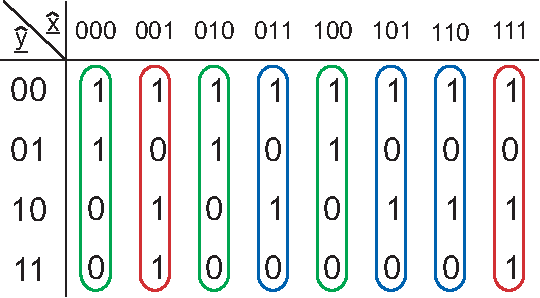
\includegraphics[width=0.3\textwidth]{Grafiken/Dekomposition1}
\end{center}
Anzahl der benötigten Variablen z: $|z|=\lceil log_2(|Z|)\rceil$\\\\
Dekompositionsbedingung: $|z| \leq |x|-1$ bzw. $|Z|\leq \frac{1}{2}|X|$

\subsection*{Schritt 2}
Konstruktion der Dekompositionsfunktion\\\\
$\underline{z}=\underline{h}(\underline{x})$ Dekompositionsfunktion\\ \\
(Willkürliche) Zuordnung von Belegungen ($\hat{z}_1,\hat{z}_2,...$):
\begin{center}
\begin{tabular}{|c|c|c|}
\hline $\underline{\hat{x}}\in X$ & $f(\underline{\hat{x}}, \underline{y})$ & $\underline{\hat{z}}$ \\ 
\hline ${\color{green}000,010,100}$ & $\overline{y}_1$ & $00$ \\ 
\hline ${\color{red}001,111}$ & $y_1+\overline{y}_2$ & $10$ \\ 
\hline ${\color{blue}011,101,110}$ & $\overline{y}_2$ & $11$ \\ 
\hline 
\end{tabular}
\end{center}
\begin{tabbing}
$z_1=$ \=${\color{red}\overline{x}_1\cdot \overline{x}_2\cdot x_3}+{\color{red}x_1\cdot x_2\cdot x_3}+{\color{blue}\overline{x}_1\cdot x_2\cdot x_3}+{\color{blue}x_1\cdot \overline{x}_2\cdot x_3}+$\\
\>${\color{blue}x_1\cdot x_2\cdot \overline{x}_3}=...=x_1\cdot x_2+x_3$\\
$z_2={\color{blue}\overline{x}_1\cdot x_2\cdot x_3}+{\color{blue}x_1\cdot \overline{x}_2\cdot x_3}+{\color{blue}x_1\cdot x_2\cdot \overline{x}_3}$
\end{tabbing}

\subsection*{Schritt 3}
Konstruktion der Kompositionsfunktion\\\\
$w=g(\underline{z},\underline{y})$ Kompositionsfunktion\\\\
$w=\overline{z}_1\cdot \overline{z}_2\cdot \overline{y}_1+z_1\cdot \overline{z}_2\cdot (y_1+\overline{y}_2\cdot)+z_1\cdot z_2\cdot \overline{y}_2$\\
$w=...=\overline{z}_1\cdot \overline{z}_2\cdot \overline{y}_1+z_1\cdot \overline{z}_2\cdot y_1+z_1\cdot\overline{y}_2$

\subsection*{Graphische Darstellung}
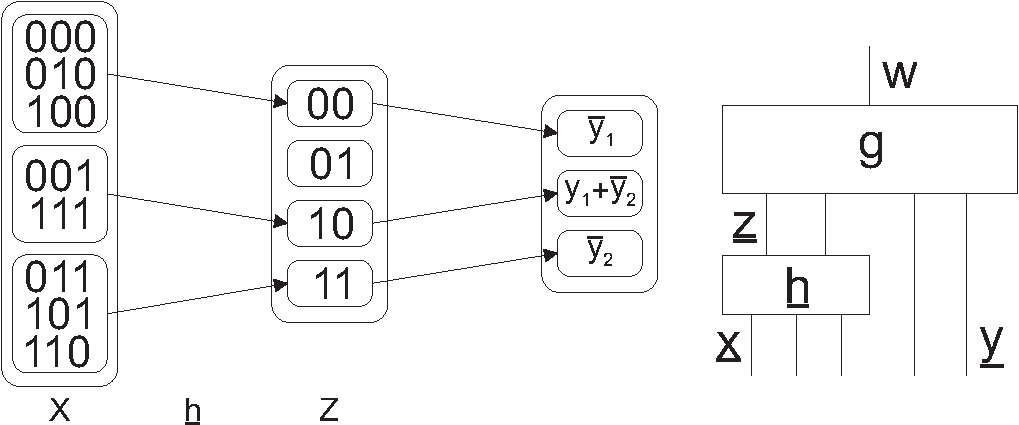
\includegraphics[width=0.45\textwidth]{Grafiken/Dekomposition2}

\section*{Finite state machine (FSM)}
FSM$=(S,I,O,\delta,\lambda,S^0)$
$S$ endliche Zustandsmenge, $I$ Menge der Eingangsmuster, $O$ Menge der Ausgangsmuster, $\delta$ Zustandsübergangsfunktion, $\lambda$ Ausgangsfunktion, $S^0\in S$ Anfangszustand

\subsection*{Zustandsminimierung}
\begin{enumerate}
	\item Eleminieren nicht erreichbarer Zustände
	\item Zusammenfassen äquivalenter Zustände
\end{enumerate}
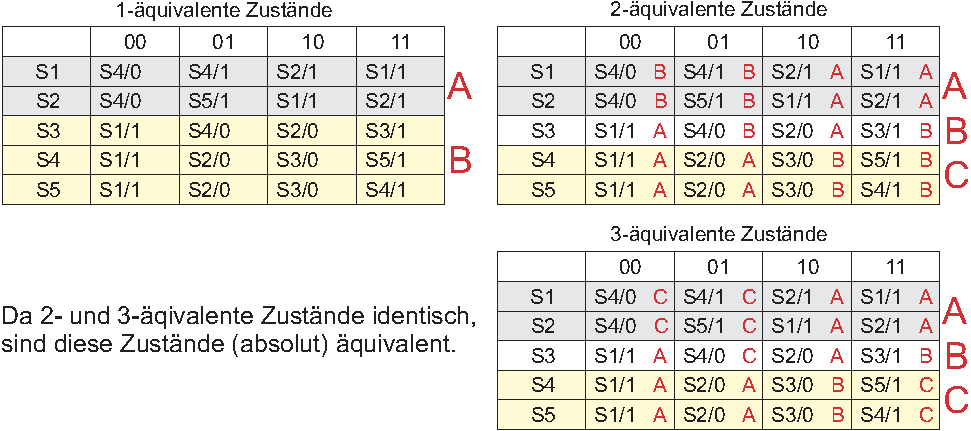
\includegraphics[width=0.5\textwidth]{Grafiken/Zustandsminimierung}

\subsection*{Realisierung}
\begin{center}
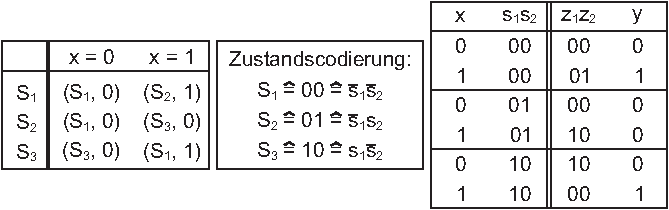
\includegraphics[width=0.45\textwidth]{Grafiken/FSM-Realisierung}
\end{center}
$y=x\cdot \overline{s}_1\cdot \overline{s}_2+x\cdot s_1\cdot \overline{s}_2 = x\cdot \overline{s}_2$\\
$z_1=x\cdot \overline{s}_1\cdot s_2+\overline{x}\cdot s_1\cdot \overline{s}_2$\\
$z_2=x\cdot \overline{s}_1\cdot \overline{s}_2$

\section*{Logiksimulation}
Ereignis: Wertänderung eines Signals\\
Ereignis: $E=(z, \val(z,t_{exe}),t_{gen},t_{exe})$\\
Laufzeitabhängige Effekte:
\begin{enumerate}
	\item Race: "Wettlauf" von Signalwertänderungen auf Leitungen vor einem gemeinsamen Knoten (Gatter)
	\item Hazard: (Spike, Glitch) Signalwertverlauf, der der reinen Logikfunktion der Schaltung widerspricht und nur durch die Verzögerungszeiten entsteht.
\end{enumerate}
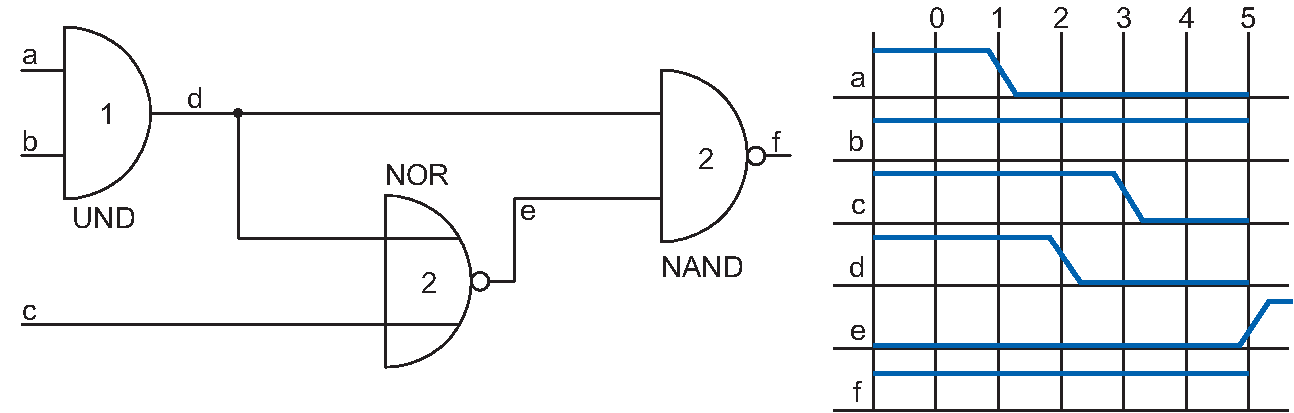
\includegraphics[width=0.5\textwidth]{Grafiken/Logiksimulation}
\\ \\
\begin{tabular}{@{}|c|c|c|c|c|c|c|p{2.3cm}|p{2cm}|@{}}
\hline t & a & b & c & d & e & f & ausgewertete Elemente & neue Events* \\
\hline 0 & 1 & 1 & 1 & 1 & 0 & 1 & init & (a,'0',0,1), (c,'0',0,3) \\ 
\hline 1 & 0 &  &  &  &  &  & AND & (d,'0',1,2) \\ 
\hline 2 &  &  &  & 0 &  &  & NAND, NOR&  \\ 
\hline 3 &  &  & 0 &  &  &  & NOR & (e,'1',3,5) \\ 
\hline 5 &  &  &  &  & 1 &  & NAND &  \\ 
\hline 
\end{tabular}\\\\
*(signal, value, $t_{gen}$,$t_{exe}$)

\section*{VHDL}
{\small \textbf{ENTITY Bausteinname IS}}\\
Definiert die Schnittstelle einer Logik\\\\
{\small \textbf{PORT (Schnittstelle)}}\\
Definiert Ein- und Ausgänge\\\\
{\small \textbf{ARCHITECTURE ... OF ... IS}}\\
Beschreibt den internen Aufbau\\\\
{\small \textbf{PROCESS (Signalliste)}}\\
Alle Prozesse laufen nebeneinander ab\\\\
{\small \textbf{COMPONENT Gattername}}\\
Beschreibt eine interne Komponente

\section*{Testverfahren}
\subsection*{Begriffe}
\textbf{Fehlerhafte Schaltung}: $y_\mu$\\
\textbf{Fehlergruppe}: Menge aller erkannten Fehler von Test $t_v$
\textbf{Fehleranzahl} = $2\cdot$ Signalanzahl\\
\textbf{Testgruppe}: Menge aller Tests die Fehler $f_\mu$ erkennen\\
\textbf{Testmenge}: Enthaltene Tests erkennen alle angenommenen Fehler\\
\textbf{Fehlerüberdeckung}: Vereinigung der Fehlergruppen enthält alle angenommenen Fehler\\\\
\textbf{Fehlererkennung}: $t_vRf_\mu=y(\underline{x}_v) \oplus y_\mu(\underline{x}_v)=1$\\\\
\textbf{Fehlerunterscheidung}: $y_\mu(\underline{x}_v) \oplus y_\kappa(\underline{x}_v)=1$\\\\
Zwei einzelne Fehler sind nicht unterscheidbar, wenn deren Testgruppen gleich sind

\subsection*{Boolesche Differenz}
$y_z=y(z,\underline{x}) \oplus y(\overline{z},\underline{x})$\\
$y_z=y(z=1) \oplus y(z=0)$

\subsubsection*{Rechenregeln}
\begin{enumerate}
	\item $y_x=0$ falls $y\neq f(x)$
	\item $y_y=1$
	\item $(\overline{y})_x=y_x$
	\item $(z \oplus w)_x=z_x\oplus w_x$
	\item $(z\cdot w)_x=z\cdot w_x\oplus z_x\cdot w \oplus z_x\cdot w_x$
	\item $(z+w)_x=\overline{z}\cdot w_x\oplus z_x\cdot \overline{w} \oplus z_x\cdot w_x$
	\item Falls $y=y(z(x)) : y_x=y_z\cdot z_x$
	\item $(y_z)_w=(y_w)_z$
\end{enumerate}	

\subsubsection*{Test}
$z/0=z\cdot y_z=1$\\
$z/1=\overline{z}\cdot y_z=1$

\subsubsection*{Fehlerbelegung (Einstellbarkeit)}
$z/0:z(\underline{x})=1$\\
$z/1:z(\underline{x})=0$

\subsubsection*{Sensibilisierungsbelegung (Beobachtbarkeit)}
$y_z(\underline{x})=1$

\subsubsection*{Strukturbezogene Berechnung der BD}
Redeweisen für $y_x$:
\begin{itemize}
	\item BD von y nach x (Boolean Difference)
	\item Beobachtbarkeit von x an y (Observability)
	\item Empfindlichkeit von y gegen x (Sensitivity)
\end{itemize}
Redeweisen für $y_x=1$:
\begin{itemize}
	\item y ist von x funktionell abhängig
	\item Fehlbelegung an x $\Rightarrow$ Fehlbelegung an y
	\item Einfachfehler an x an y beobachtbar
\end{itemize}

\begin{enumerate}[label=,leftmargin=0mm]
	\item $y_x=y(x)\oplus y(\overline{x})$
	\item $y\oplus y_x=y(\overline{x})=z(\overline{x}) \circ w(\overline{x})$
	\item \fbox{$y\oplus y_x=(z\oplus z_x) \circ (w\oplus w_x)$}
	\item $y_x=\left[(z\oplus z_x) \circ (w\oplus w_x)\right]\oplus\left[z\circ w\right]$
	\item \fbox{$y_x=y_z\cdot z_x\cdot\overline{w_x}+y_w\cdot w_x\cdot\overline{z_x}+z_x\cdot w_x\cdot\left[\overline{z}\circ\overline{w}\oplus z\circ w\right]$}
	\item $y_x=\left[(z\oplus z_x) \circ (w\oplus w_x) \circ (v\oplus v_x)\right]\oplus\left[z\circ w\circ v\right]$
	\item 
\end{enumerate}

\subsection*{Pfadsensibilisierung}
\begin{enumerate}
	\item $y_z\cdot z_x\cdot \overline{w_x}=1 : $ Einfachfehlerpfad x-z-y
	\item $y_w\cdot w_x\cdot \overline{z_x}=1 : $ Einfachfehlerpfad x-w-y
	\item $z_x\cdot w_x\cdot\left[\overline{z}\circ\overline{w}\oplus z\circ w\right]=1 : $ Mehrfachpfadsensibilisierung
	\item $z_x\cdot w_x\cdot\overline{\left[\overline{z}\circ\overline{w}\oplus z\circ w\right]}=1 : $ Selbstmaskierung
\end{enumerate}

\subsection*{Fehlerbaumkonstruktion}
\begin{enumerate}
	\item Gut-Simulation der Eingangsbelegung
	\item Fehler x/v mit $v=\overline{\val(x)}$ einstellbar.
	\item Welche Eingänge wirken sich auf das jeweilige Gatter aus?
		$\Rightarrow$ Mit Punkt und dicker Linie markieren
	\item Fan-outs auftrennen. Die relevanten Fan-outs sind diejenigen, die sich bei verändertem Signalwert auf den Ausgang auswirken.
	\item Menge $S^0$: Alle Signale, die im Fehlerbaum eine ,,Verbindung zum Ausgang'' haben.
	\item Menge $F^t$: Alle Fehler, die sich auf den Ausgang auswirken.
\end{enumerate}

\subsection*{D-Algorithmus}
$D$: '1' im fehlerfreien Fall, '0' im fehlerhaften Fall
$\overline{D}$: '0' im fehlerfreien Fall, '1' im fehlerhaften Fall
D-Kette $V_D$: Einfach-/Mehrfachfehlerpfad von x zum Ausgang y\newline
\begin{tabular}{cc}
\begin{tabular}{c|ccccc}
$\cdot$ & 0 & 1 & $X$ & $D$ & $\overline{D}$ \\ 
\hline 0 & 0 & 0 & 0 & 0 & 0 \\ 
1 & 0 & 1 & $X$ & $D$ & $\overline{D}$ \\ 
$X$ & 0 & $X$ & $X$ & $X$ & $X$ \\ 
$D$ & 0 & $D$ & $X$ & $D$ & 0 \\ 
$\overline{D}$ & 0 & $\overline{D}$ & $X$ & 0 & $\overline{D}$ \\  
\end{tabular} &        
\begin{tabular}{c|ccccc}
$+$ & 0 & 1 & $X$ & $D$ & $\overline{D}$ \\ 
\hline 0 & 0 & 1 & $X$ & $D$ & $\overline{D}$ \\ 
1 & 1 & 1 & 1 & 1 & 1 \\ 
$X$ & $X$ & 1 & $X$ & $X$ & $X$ \\ 
$D$ & $D$ & 1 & $X$ & $D$ & 1 \\ 
$\overline{D}$ & $\overline{D}$ & 1 & $X$ & 1 & $\overline{D}$ \\  
\end{tabular} \\\\
\begin{tabular}{c|ccccc}
$\oplus$ & 0 & 1 & $X$ & $D$ & $\overline{D}$ \\ 
\hline 0 & 0 & 1 & $X$ & $D$ & $\overline{D}$ \\ 
1 & 1 & 0 & $X$ & $\overline{D}$ & $D$ \\ 
$X$ & $X$ & $X$ & $X$ & $X$ & $X$ \\ 
$D$ & $D$ & $\overline{D}$ & $X$ & 0 & 1 \\ 
$\overline{D}$ & $\overline{D}$ & $D$ & $X$ & 1 & 0 \\ 
\end{tabular} &
\begin{tabular}{c|c}
$a$ & $\overline{a}$ \\
\hline 0 & 1 \\
1 & 0 \\
$X$ & $X$ \\
$D$ & $\overline{D}$ \\
$\overline{D}$ & $D$ \\
\end{tabular} 
\end{tabular}\newline
F: Fehlerbelegung; S: Sensibilisierung
I: Implikation; O: Optionale Wertzuweisung

\subsection*{Globale Implikation}
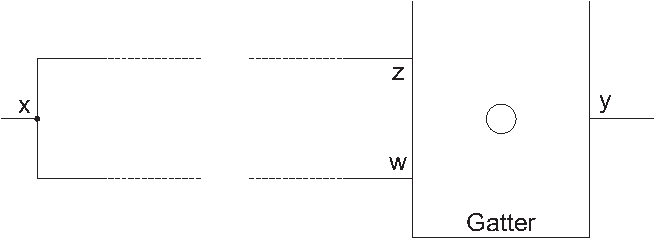
\includegraphics[width=0.24\textwidth]{Grafiken/Lernkriterium}

\subsubsection*{Lernprozedur (Kontrapositionsgesetz)}
$\widehat{x} \Rightarrow \widehat{y}$ genau dann, wenn $\overline{\widehat{y}} \Rightarrow \overline{\widehat{x}}$\\
Es sollen nur globale Implikationen gelernt werden.\\\\
Nur lernenswert falls bei \textbf{Vorwärtsimplikation} gilt:
$y_z\cdot y_w=1$

\subsection*{Einstellbarkeitsmaße(Controllability)}
$C_0$: Nulleinstellbarkeit; $C_1$: Einseinstellbarkeit
$x$ Eingangsvariable $\Rightarrow C_0(x)=C_1(x)=0.5$\\
Bei mehreren Alternativen zur Sicherstellung eines Signalwertes wird derjenige mit dem größten Einstellbarkeitsmaß ausgewählt (Nur bei Baumstrukturen exakt!).
\\\\
Lizenz: CC BY-NC-SA 3.0\\
\url{http://creativecommons.org/licenses/by-nc-sa/3.0/de/}

\end{document}








